\documentclass{article}

% if you need to pass options to natbib, use, e.g.:
%     \PassOptionsToPackage{numbers, compress}{natbib}
% before loading neurips_data_2023

% ready for submission
\usepackage{neurips_2025}

% to compile a preprint version, add the [preprint] option, e.g.:
%     \usepackage[preprint]{neurips_data_2023}
% This will indicate that the work is currently under review.

% to compile a camera-ready version, add the [final] option, e.g.:
%     \usepackage[final]{neurips_data_2023}

% to avoid loading the natbib package, add option nonatbib:
%    \usepackage[nonatbib]{neurips_data_2023}

% Submissions to the datasets and benchmarks are typically non anonymous,
% but anonymous submissions are allowed. If you feel that you must submit 
% anonymously, you can compile an anonymous version by adding the [anonymous] 
% option, e.g.:
%     \usepackage[anonymous]{neurips_data_2023}
% This will hide all author names.

\usepackage[utf8]{inputenc} % allow utf-8 input
\usepackage[T1]{fontenc}    % use 8-bit T1 fonts
\usepackage{hyperref}       % hyperlinks
\usepackage{url}            % simple URL typesetting
\usepackage{booktabs}       % professional-quality tables
\usepackage{amsfonts}       % blackboard math symbols
\usepackage{nicefrac}       % compact symbols for 1/2, etc.
\usepackage{microtype}      % microtypography
\usepackage{xcolor}         % colors
\usepackage{upquote}
\usepackage{fancyvrb}
\usepackage{float}


\usepackage{soul}
\definecolor{deepblue}{rgb}{0,0,0.5}
\definecolor{deepred}{rgb}{0.6,0,0}
\definecolor{deepgreen}{rgb}{0,0.5,0}

\usepackage{listings}
\usepackage{graphicx}
\usepackage{courier}
\usepackage{color}


% Improved lstListing settings based on https://gist.github.com/mpdehnel/cc43e89a09c18ef6a602
\definecolor{mygreen}{rgb}{0,0.6,0}
\definecolor{mygray}{rgb}{0.5,0.5,0.5}
\definecolor{mymauve}{rgb}{0.58,0,0.82}
\lstset{ %
  backgroundcolor=\color{white},   % choose the background color; you must add \usepackage{color} or \usepackage{xcolor}
  basicstyle=\footnotesize\ttfamily,        % the size of the fonts that are used for the code
  breakatwhitespace=false,         % sets if automatic breaks should only happen at whitespace
  breaklines=false,                 % sets automatic line breaking
  captionpos=none,                    % sets the caption-position to bottom
  commentstyle=\color{gray},    % comment style
  deletekeywords={...},            % if you want to delete keywords from the given language
  escapeinside={\%*}{*)},          % if you want to add LaTeX within your code
  extendedchars=true,              % lets you use non-ASCII characters; for 8-bits encodings only, does not work with UTF-8
  frame=single,                    % adds a frame around the code
  keepspaces=true,                 % keeps spaces in text, useful for keeping indentation of code (possibly needs columns=flexible)
  keywordstyle=\color{blue},       % keyword style
  language=Python,                 % the language of the code
  otherkeywords={*,...},            % if you want to add more keywords to the set
  numbers=left,                    % where to put the line-numbers; possible values are (none, left, right)
  numbersep=5pt,                   % how far the line-numbers are from the code
  numberstyle=\tiny\color{mygray}, % the style that is used for the line-numbers
  rulecolor=\color{black},         % if not set, the frame-color may be changed on line-breaks within not-black text (e.g. comments (green here))
  showspaces=false,                % show spaces everywhere adding particular underscores; it overrides 'showstringspaces'
  showstringspaces=false,          % underline spaces within strings only
  showtabs=false,                  % show tabs within strings adding particular underscores
  stepnumber=2,                    % the step between two line-numbers. If it's 1, each line will be numbered
  stringstyle=\color{mymauve},     % string literal style
  tabsize=2,                       % sets default tabsize to 2 spaces
  numbers=none,
  title=\lstname                   % show the filename of files included with \lstinputlisting; also try caption instead of title
}


\DeclareFixedFont{\ttb}{T1}{txtt}{bx}{n}{10} % for bold
\DeclareFixedFont{\ttm}{T1}{txtt}{m}{n}{10}  % for normal

\DeclareFixedFont{\ttbsmall}{T1}{txtt}{bx}{n}{8} % for bold
\DeclareFixedFont{\ttmsmall}{T1}{txtt}{m}{n}{8}  % for normal

% Python style for highlighting
\newcommand\pythonstyle{\lstset{
language=Python,
basicstyle=\ttm,
morekeywords={self},              % Add keywords here
keywordstyle=\ttb\color{deepblue},
emph={MyClass,__init__},          % Custom highlighting
emphstyle=\ttb\color{deepred},    % Custom highlighting style
stringstyle=\color{deepgreen},
frame=tb,                         % Any extra options here
showstringspaces=false
}}


% Python environment
\lstnewenvironment{python}[1][]
{
\pythonstyle
\lstset{#1}
}
{}

% Python for external files
\newcommand\pythonexternal[2][]{{
\pythonstyle
\lstinputlisting[#1]{#2}}}

% Python for inline
\newcommand\pythoninline[1]{{\pythonstyle\lstinline!#1!}}

% Python small style for highlighting
\newcommand\pythonsmallstyle{\lstset{
language=Python,
basicstyle=\ttmsmall,
morekeywords={self},              % Add keywords here
keywordstyle=\ttbsmall\color{deepblue},
emph={MyClass,__init__},          % Custom highlighting
emphstyle=\ttbsmall\color{deepred},    % Custom highlighting style
stringstyle=\color{deepgreen},
frame=tb,                         % Any extra options here
showstringspaces=false
}}


% Python environment
\lstnewenvironment{pythonsmall}[1][]
{
\pythonsmallstyle
\lstset{#1}
}
{}


% Bash style for highlighting
\newcommand\bashstyle{\lstset{
language=bash,
basicstyle=\ttm,
morekeywords={},              % Add keywords here
keywordstyle=\ttm,%\ttb\color{deepblue},
emph={},          % Custom highlighting
emphstyle=\ttb\color{deepred},    % Custom highlighting style
stringstyle=\color{deepgreen},
frame=tb,                         % Any extra options here
showstringspaces=false
}}


% Python environment
\lstnewenvironment{bash}[1][]
{
\bashstyle
\lstset{#1}
}
{}

% Python for external files
\newcommand\bashexternal[2][]{{
\bashstyle
\lstinputlisting[#1]{#2}}}

% Python for inline
\newcommand\bashinline[1]{{\bashstyle\lstinline!#1!}}

\newcommand{\todoAD}[1]{\color{red} [\textbf{AD: } #1]}


%\title{Minari: Facilitating Community-Based Reinforcement Learning Datasets}
\title{Minari: Infrastructure for Collaborative Reinforcement Learning Datasets}

% The \author macro works with any number of authors. There are two commands
% used to separate the names and addresses of multiple authors: \And and \AND.
%
% Using \And between authors leaves it to LaTeX to determine where to break the
% lines. Using \AND forces a line break at that point. So, if LaTeX puts 3 of 4
% authors names on the first line, and the last on the second line, try using
% \AND instead of \And before the third author name.

\author{%
  David S.~Hippocampus\thanks{Use footnote for providing further information
    about author (webpage, alternative address)---\emph{not} for acknowledging
    funding agencies.} \\
  Department of Computer Science\\
  Cranberry-Lemon University\\
  Pittsburgh, PA 15213 \\
  \texttt{hippo@cs.cranberry-lemon.edu} \\
  % examples of more authors
  % \And
  % Coauthor \\
  % Affiliation \\
  % Address \\
  % \texttt{email} \\
  % \AND
  % Coauthor \\
  % Affiliation \\
  % Address \\
  % \texttt{email} \\
  % \And
  % Coauthor \\
  % Affiliation \\
  % Address \\
  % \texttt{email} \\
  % \And
  % Coauthor \\
  % Affiliation \\
  % Address \\
  % \texttt{email} \\
}

\begin{document}

\maketitle

\begin{abstract}
The sharing and reuse of agent experience data is crucial for advancing reinforcement learning capabilities. However, existing methods are often fragmented due to inconsistent formats, inadequate documentation, and limited reproducibility. 
To address these issues, we introduce Minari, an open-source library designed to standardize the collection, sharing, and integration of reinforcement learning trajectories. Inspired by the design principles of Gym and Gymnasium, Minari offers a unified interface for working with agent experience data through a familiar and extensible API.
The library supports the entire dataset lifecycle. Researchers can collect trajectories from any environment, annotate them with metadata, manipulate and combine datasets, and share them effortlessly through integration with the HuggingFace Hub. Minari aims to establish a standard for reinforcement learning datasets that enhances interoperability, utilizing consistent naming conventions, detailed metadata, and support for multiple file formats.
Additionally, Minari is already integrated with major offline reinforcement learning frameworks. It includes a curated collection of 338 reproducible datasets across various domains, such as robotics navigation, manipulation tasks, grid navigation, text-based instruction following, Atari games, hierarchical planning tasks, and trajectories from web agents. This growing dataset collection currently offers 350K different trajectories, totaling 55M interaction steps.
By lowering the barriers to sharing and reusing agent experience data, Minari seeks to accelerate collaborative progress in offline reinforcement learning research.
\end{abstract}

\section{Introduction}

As we enter the \textit{Era of Experience} \cite{experience-era}, where learning from interactions becomes crucial for AI progress, the data generated by intelligent agents represents an increasingly valuable resource. This data encapsulates how agents interact with environments over time and the outcome of these interactions. Despite its growing importance, the sharing and reuse of agent experience remains limited and fragmented.

Three critical challenges impede progress in this domain. First, agent experience data is rarely collected or distributed in standardized formats, creating immediate barriers to interoperability. Second, when experience datasets are shared, they are typically not reproducible, have inconsistent documentation, or environment-specific assumptions that complicate integration and reuse. Third, combining datasets from different sources into a coherent and usable form is particularly challenging, requiring significant manual effort and domain-specific adjustments. This lack of standardization impedes collaboration and slows down progress in the field. 

To address these limitations, we introduce Minari, an open-source library designed to streamline the collection, sharing, and ingestion of agent experience. Minari provides a unified interface for reinforcement learning datasets inspired by the design philosophy of Gym and Gymnasium \cite{gym, gymnasium}, offering a familiar and extensible API for interacting with trajectory data. A simple example usage is given in Figure ~\ref{fig:code}, and is described in detail in Sect.~\ref{sec:library_features}. Our primary objective is to establish a robust standard for reinforcement learning datasets that enhances interoperability, improves reproducibility, and facilitates collaboration across the research community.

Minari supports the full dataset lifecycle: researchers can collect trajectories from any environment, annotate and manipulate them, and upload them to the HuggingFace Hub\footnote{https://huggingface.co} or other cloud platforms with a single command. Datasets can also be downloaded, inspected, and combined via a simple command-line interface or Python API. This enables seamless integration with training libraries and workflows, allowing users to swap or merge datasets by changing a single line of code.

By standardizing experience data and lowering the barrier to sharing and reuse, Minari paves the way for large scale, collaborative progress in reinforcement learning.

\begin{figure}[t]
    \centering
   \begin{pythonsmall}
  import minari
  import gymnasium as gym
  env = gym.make('CartPole-v1')
  env = minari.DataCollector(env, record_infos=True)
  ... # Step through environment as usual
  dataset = env.create_dataset("cartpole/test-v0")\end{pythonsmall}
   \begin{pythonsmall}
  import minari
  dataset = minari.load_dataset('D4RL/door/human-v2', download=True)
  episodes = dataset.sample_episodes(n_episodes=5) # Sample 5 episodes
  env = dataset.recover_environment() # Optionally recover data collection env\end{pythonsmall}
  \caption{Two examples of Minari usage. \textbf{Top:} Creating a Minari dataset using the Gymnasium wrapper. Non-Gymnasium environments are also supported and can be created manually via \lstinline|minari.create_dataset_from_buffers()|. \textbf{Bottom:} Loading an existing dataset (local or remote). In many cases one can instead directly use one of the integrations with existing Offline RL  libraries described in Sec.~\ref{sec:integrations}.}
    \label{fig:code}
\end{figure}

\section{Related work}
Several open-source libraries inspired and laid the foundation for the development of Minari.

\paragraph{RLDS} The Reinforcement Learning Datasets (RLDS) \cite{rlds} provides a framework for storing and manipulating RL trajectories using TensorFlow-based data structures. RLDS introduced a standardized schema for trajectory data and offers efficient operations for data manipulation, from which we take inspiration while developing Minari. However, its tight coupling with the TensorFlow ecosystem limits its accessibility.

\paragraph{D4RL} The Dataset for Data-Driven Deep Reinforcement Learning (D4RL) \cite{d4rl} was one of the first major benchmarks for offline RL, providing a collection of tasks and pre-recorded datasets to evaluate algorithms. While D4RL made significant contributions by establishing baseline performance metrics across various domains, its datasets are tied to specific environment versions and cannot be reliably reproduced. Additionally, D4RL does not offer tools for practitioners to create and share their datasets. Minari addresses these limitations by providing a comprehensive toolset for dataset creation, manipulation, and distribution while ensuring version compatibility and reproducibility.

\paragraph{RL Unplugged} RL Unplugged \cite{rlunplugged} represents another significant contribution to offline reinforcement learning research, providing a diverse suite of tasks and corresponding datasets across domains including DeepMind Control Suite \cite{deepmindcontrolsuite}, and Atari games. Similar to D4RL, it enables benchmarking of offline RL algorithms but with a stronger emphasis on challenging exploration scenarios. However, it shares D4RL's limitations regarding reproducibility and extensibility, as datasets are provided as fixed collections without standardized tools for researchers to create compatible datasets of their own.

\paragraph{LeRobot} LeRobot \cite{lerobot} is an open-source library that provides models, datasets, and tools for robotics in PyTorch. Although LeRobot provides valuable resources to the robotics community, its focus remains specifically on real-world robotics applications rather than general agent learning. On the other hand, Minari provides a generalized framework designed for all types of intelligent agents.

\paragraph{HuggingFace Hub} The HuggingFace Hub has emerged as a central repository for machine learning models and datasets, particularly in the natural language processing domain. Its infrastructure for version control, documentation, and community collaboration has positively impacted resource sharing in deep learning. While not specifically designed for reinforcement learning data, HuggingFace Hub provides valuable infrastructure for hosting datasets. Minari leverages this infrastructure by implementing native integration with the Hub, enabling researchers to publish, version, and download reinforcement learning datasets.

\subsection{Library integrations}
\label{sec:integrations}
Minari is natively supported by many of the most popular libraries supporting offline RL training, making it easy to use Minari datasets in training pipelines. We list here the libraries that natively integrate Minari.

\paragraph{TorchRL} TorchRL \cite{torchrl} is a PyTorch-based library for reinforcement learning that provides modular and flexible tools to build and train RL agents. It supports a wide range of environments and integrates tightly with the PyTorch ecosystem. The library is designed to be scalable and customizable for both research and production applications.

\paragraph{AgileRL}
AgileRL \cite{agilerl} is an open-source library designed to automate the process of designing and optimizing reinforcement learning agents. It focuses on enabling fast experimentation by using meta-learning and population-based training to evolve agent architectures and hyperparameters. AgileRL is particularly suited for practitioners who want to quickly prototype high-performing agents without deep RL expertise.

\paragraph{D3RLPY}
d3rlpy \cite{d3rlpy} is a data-driven deep reinforcement learning library. It provides implementations of state-of-the-art offline RL algorithms like CQL \cite{CQL}, BCQ \cite{BCQ}, and TD3+BC \cite{TD3+BC} with easy-to-use APIs built on top of PyTorch.

\section{Library features}
\label{sec:library_features}

\subsection{Dataset standards}
Minari establishes a comprehensive standard for reinforcement learning datasets that promotes interoperability and reproducibility. The library adopts a consistent and descriptive naming convention for datasets using the following syntax:
\begin{verbatim}
    namespace/environment/dataset_name-v(version)
\end{verbatim}
where the \verb|namespace| enables logical grouping of related datasets, \verb|environment| indicates the name of the data source environment, \verb|dataset| names describe the content, and version numbers track iterations; only the dataset name is mandatory. For example, a human demonstration dataset from the \textit{AdroitHandDoor} environment would be identified as \verb|door/human-v0|, or if grouped under a namespace like D4RL, as \verb|D4RL/door/human-v0|.

Each dataset is stored with rich metadata that captures essential information about it. The default dataset metadata includes identifiers, the total number of episodes and steps, data source environment specifications (if available), action and observation spaces, code references, authorship information, algorithm details, and version compatibility requirements for full reproducibility. Additionally, episode-level metadata provides statistical summaries of rewards (maximum, minimum, mean, standard deviation, and sum), enabling efficient filtering and selection of episodes for training or evaluation.

The core data encapsulates all information from the agent's interaction with the environment. This is structured as a sequence of episodes, where each episode includes observations, actions, rewards, termination and truncation flags, and optional information dictionaries. The flexible format accommodates various types of actions and observations while maintaining strict consistency in structure, ensuring that datasets can be easily preprocessed and combined. This standardization is particularly valuable for offline reinforcement learning, where algorithms often require consistent data representations across diverse environments and tasks.

Minari supports multiple file formats seamlessly integrated through the Python library's unified API. Specifically, it offers HDF5 formatting for quick plug-and-play with small datasets, as well as Arrow and Parquet formats optimized for large-scale distributed training.

\subsection{Minari software package}
\begin{table}[]
    \centering
    \begin{tabular}{cc}
    \toprule
    \textbf{Command name} & \textbf{Description}\\
    \midrule
     \bashinline{list local} & List Minari datasets in local storage. \\
     \bashinline{list remote} & List Minari datasets in remote storage. \\
     %\hline
     \bashinline{show} & Describe a local or remote dataset, and its environment. \\
     %\hline
     \bashinline{delete} & Delete datasets from local database. \\
     %\hline
     \bashinline{download} & Download Minari datasets from remote server.\\
     %\hline
     \bashinline{upload} & Upload Minari datasets to the specified remote server. \\
     %\hline
     \bashinline{combine} & Combine multiple datasets into a single dataset.\\
     \bottomrule
    \end{tabular}
    \caption{List of available commands in the Minari command line interface, along with their description. To use a command append minari before the command name, e.g. \textit{minari list local}; \textit{-\,-help} can be used for more information.}
    \label{tab:cli}
\end{table}

Minari offers a comprehensive set of features to create, read, manipulate, and share reinforcement learning datasets. The library is designed with a focus on ease of use while maintaining the flexibility needed for diverse research applications. It can be downloaded easily from the Python Package Index (PyPI), making installation straightforward across various platforms and environments.

For convenience, specifically for common one-time operations on datasets such as download or merge, Minari provides a set of commands that are executable directly from the terminal. We provide a complete list of these commands in Table \ref{tab:cli}, enabling researchers to perform essential dataset operations without writing Python code.
To create a new dataset, we provide two primary methods: using a Gymnasium wrapper, which automatically collects the data from the environment during agent interaction (see Fig.~\ref{fig:code}), or by adding data to a buffer object, which can then be serialized to disk in the Minari format. The Gymnasium wrapper approach is particularly useful for recording live agent experiences with minimal code changes, while the buffer approach offers more control over the dataset creation process and enables the integration of data from non-Gymnasium environments or external sources.
% TODO: add image JPEG encoding

The library also provides utilities for dataset manipulation, allowing researchers to filter episodes based on specific criteria, combine datasets from different sources, and efficiently shuffle the data.
Minari's integration with the HuggingFace Hub enables seamless sharing of datasets with the research community. Researchers can publish their datasets with a single command, making their experimental data available for verification and extension. Similarly, published datasets can be downloaded and used in experiments with minimal effort, promoting reproducibility and building upon existing work.

\subsection{Improving reproducibility in Offline RL}

Reproducibility represents a crucial challenge in reinforcement learning \cite{hendersonDeepReinforcementLearning2019}, particularly in offline RL where dataset variability introduces additional complexity. Discrepancies in the environment, even minor ones, can create a misalignment between data generation and evaluation conditions. Minari addresses these reproducibility challenges through three key design innovations.

First, its \pythoninline{dataset.recover_environment()} utility reconstructs not only the original Gymnasium environment that generated the dataset but also preserves the applied wrappers that modified environmental parameters. Second, Minari automatically preserves generation seeds, even if the user does not explicitly set them, ensuring consistent data recollection. 
Finally, variations in the environment can also be introduced by changes in the underlying software implementation, especially for physics-based environments such as MuJoCo~\cite{mujoco} which use numerical integration to model rigid-body dynamics. To help control this, pip requirements can be specified during the creation of a dataset, and Minari will automatically check to ensure that the current set of installed packages is compatible with the requirement specification.

\section{Available datasets}

Minari is distributed with a comprehensive collection of curated datasets, accessible through our HuggingFace repository. There are currently 336 diverse datasets totaling 56GB in our remote repository. To ensure complete reproducibility, we provide the dataset generation scripts in a public GitHub repository\footnote{https://github.com/Farama-Foundation/minari-dataset-generation-scripts}. The following section catalogs the currently available datasets, each of which is thoroughly documented with specifications and usage guidelines in the official documentation\footnote{https://minari.farama.org}. These resources enable researchers to easily replicate and extends our datasets.

\subsection{D4RL}
\begin{figure}[t!]
    \centering
    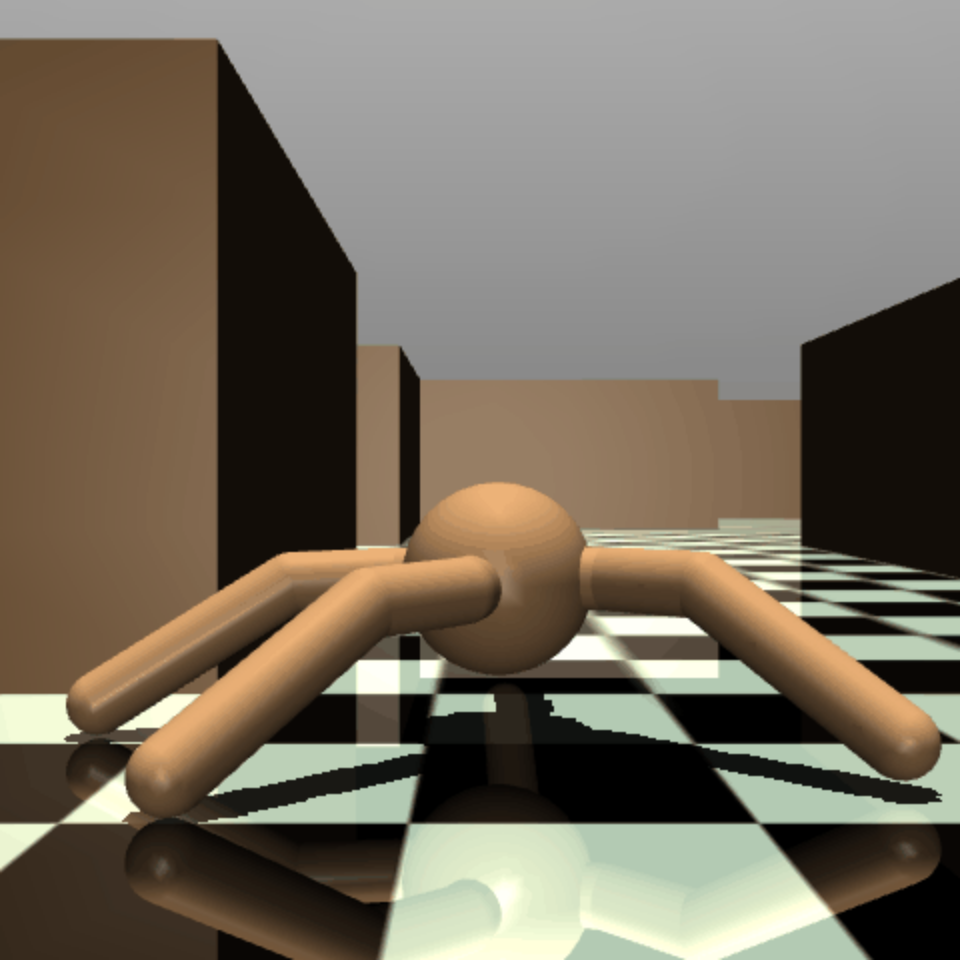
\includegraphics[width=0.18\linewidth]{figs/d4rl_ant.png}
    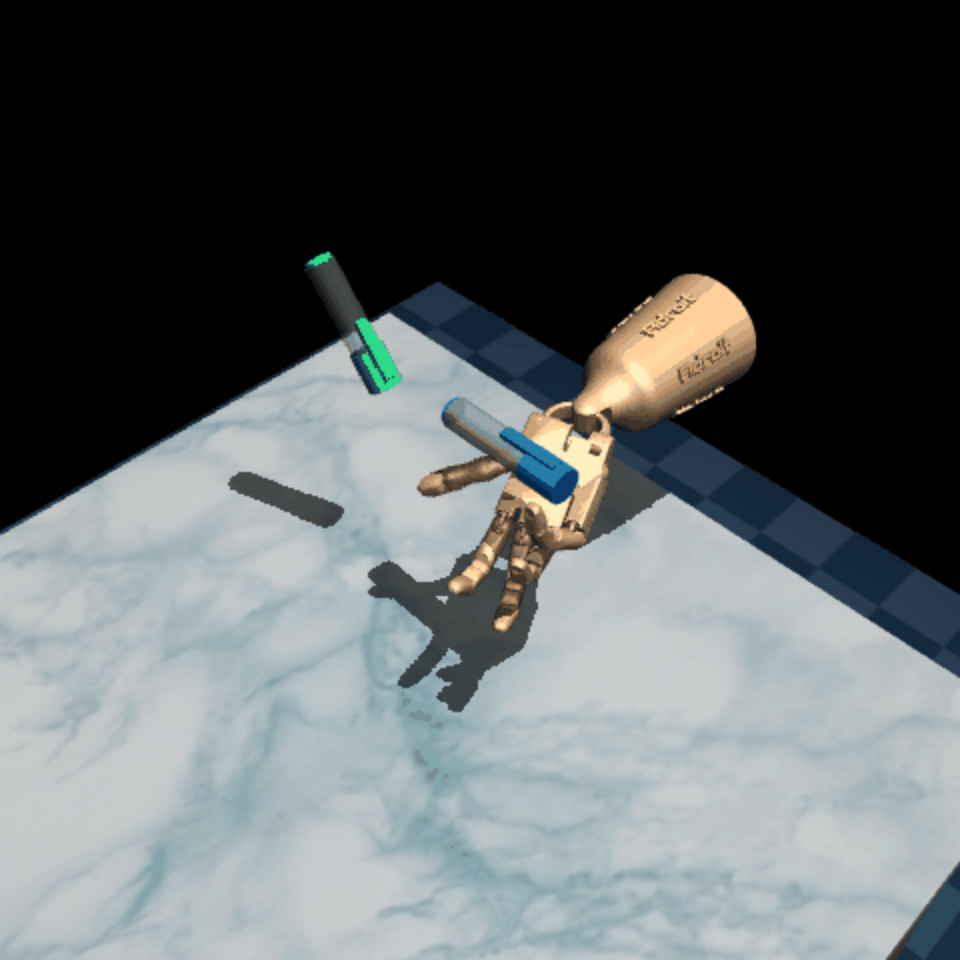
\includegraphics[width=0.18\linewidth]{figs/d4rl_pen.png}
    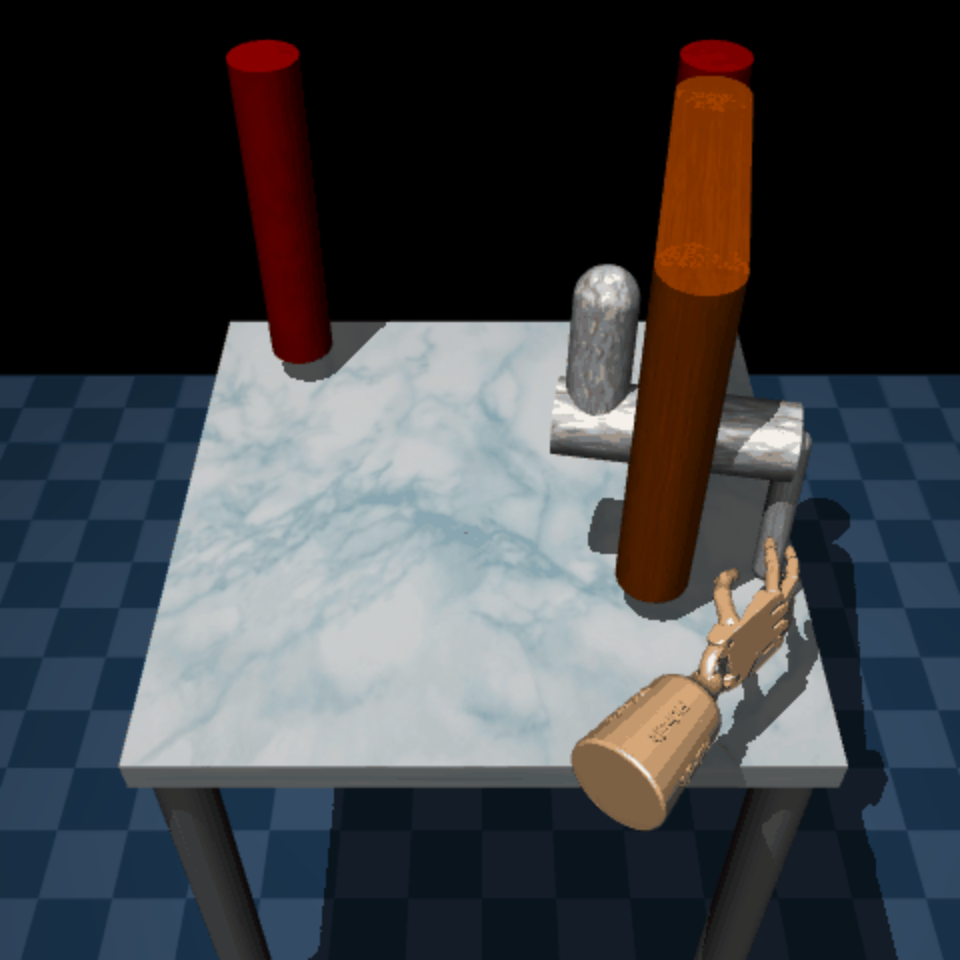
\includegraphics[width=0.18\linewidth]{figs/d4rl_door.png}
    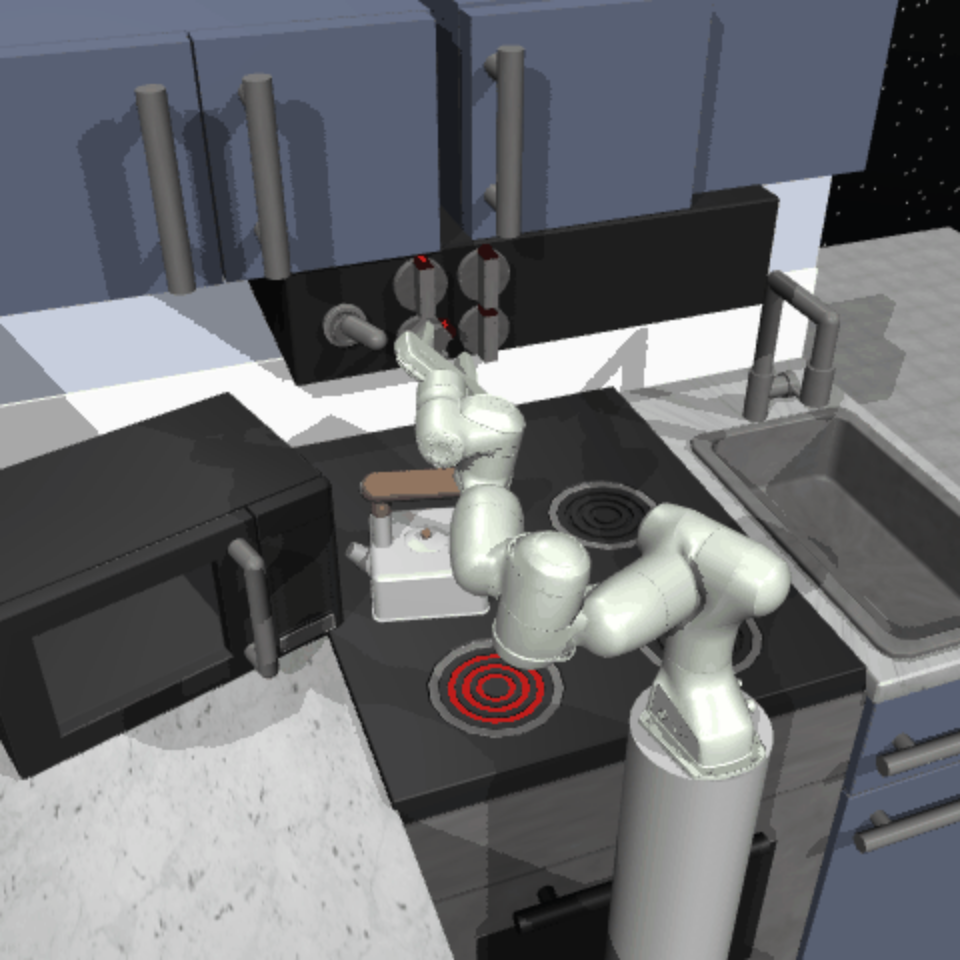
\includegraphics[width=0.18\linewidth]{figs/d4rl_kitchen.png}
    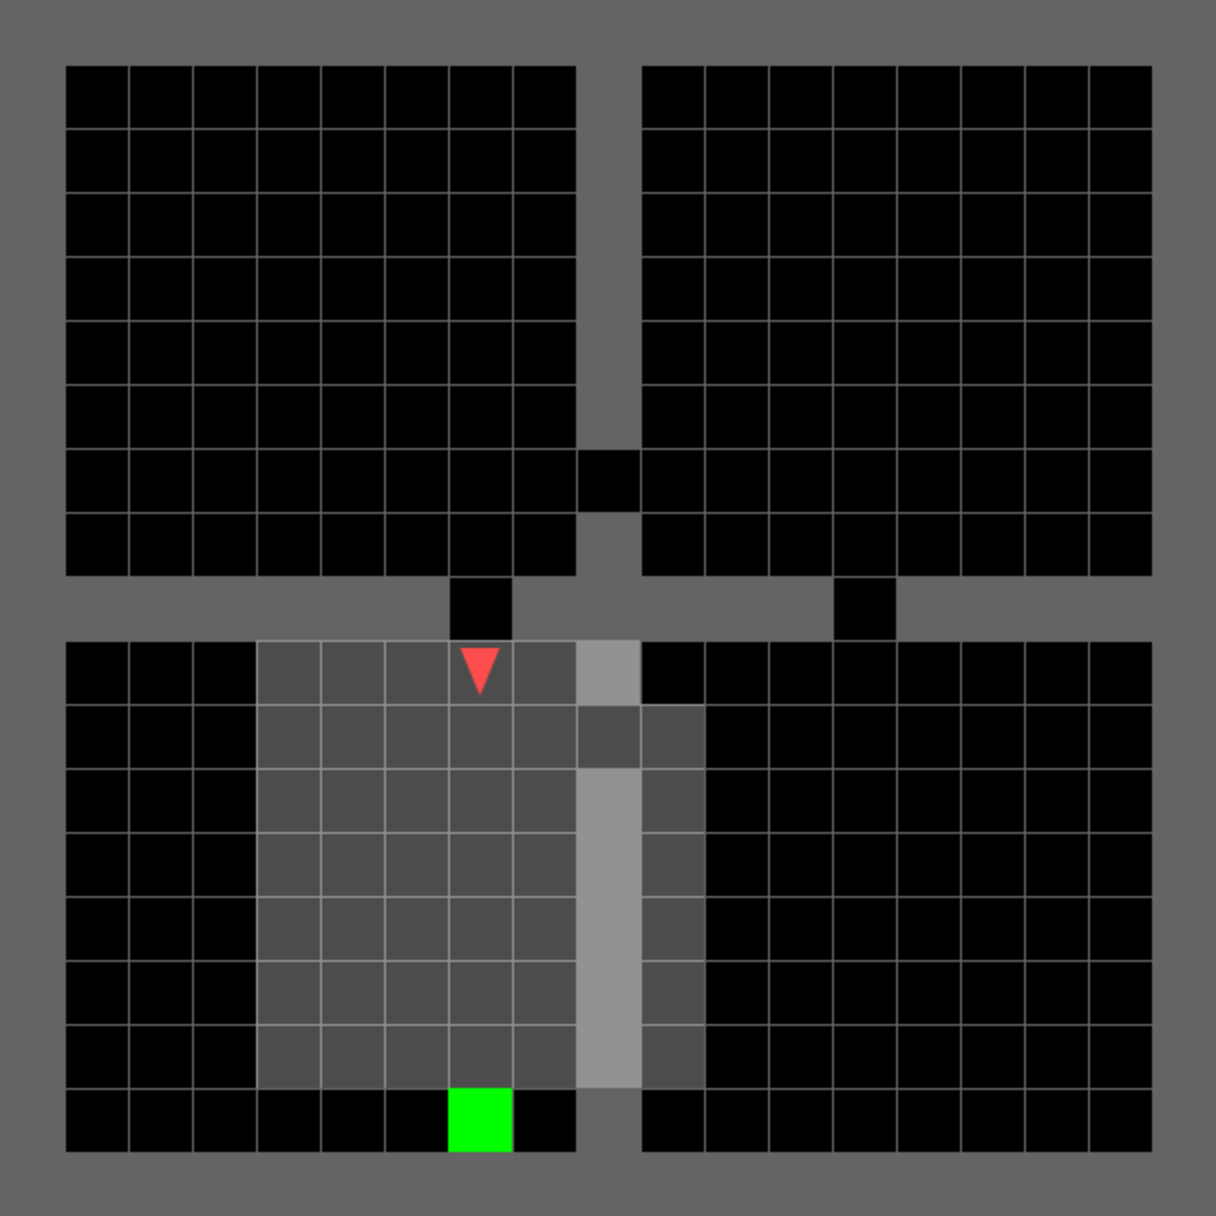
\includegraphics[width=0.18\linewidth]{figs/d4rl_minigrid.png}
    \caption{D4RL datasets: \textsc{Ant}, \textsc{Pen}, \textsc{Door}, \textsc{Kitchen}, and \textsc{MiniGrid} environments (left to right).}
    \label{fig:dr4l}
\end{figure}
The D4RL dataset group contains a reproduction of the datasets from the D4RL benchmark \cite{d4rl}. For reproducibility, we regenerated the datasets using the same principles. The collection includes:
\begin{itemize}
    \item  \textbf{Ant Maze}: Navigation tasks with an 8-DoF Ant quadruped robot following waypoints generated by a Q-value iteration planner, with >80\% success rate. This includes 6 datasets across different maze configurations.
    \item \textbf{Point Maze}: A force-actuated ball navigating to random goal locations using a non-Markovian policy with Q-value iteration planning and PD controller. This includes 8 datasets across 4 different maze configurations, and 2 different rewards type.
    \item \textbf{Manipulation Tasks}: Four high-dimensional (24-DoF) robotic hand manipulation environments, as in \cite{d4rl-pen}:
\begin{itemize}
    \item \textbf{Pen}: Manipulating a pen to reach specific orientations
    \item \textbf{Door}: Opening a door with a robotic hand
    \item \textbf{Hammer}: Using a hammer tool to drive a nail
    \item \textbf{Relocate}: Moving a ball to a target position
\end{itemize}
    For each of them, we created 3 different datasets: one derived from human demonstrations from the original paper, one generated by a trained RL policy, and one developed through imitation learning from the combined previous two datasets, as in D4RL.
    \item \textbf{Kitchen}: Datasets originally from \cite{relaypolicylearning}, where a Franka robot interacts with kitchen objects to reach desired configurations by completing 4 subtasks: opening the microwave, moving the kettle, flipping a light switch, and sliding open a cabinet door. Following D4RL, we created three dataset variants: (1) "expert" trajectories where all four tasks are completed in sequence, (2) "mixed" trajectories where all target subtasks are completed alongside additional tasks, and (3) "partial" trajectories containing various subtask combinations but never all four target subtasks in sequence.
    \item \textbf{Minigrid four rooms} As in D4RL, we generate two datasets for the Minigrid \cite{minigrid} four rooms environment, where an agent needs to navigate in a grid environment and reach a goal. The first dataset is generated using a random policy, while the second one is generated with an optimal policy using value iteration.
\end{itemize}

\subsection{MuJoCo}
\begin{figure}[t!]
    \centering
    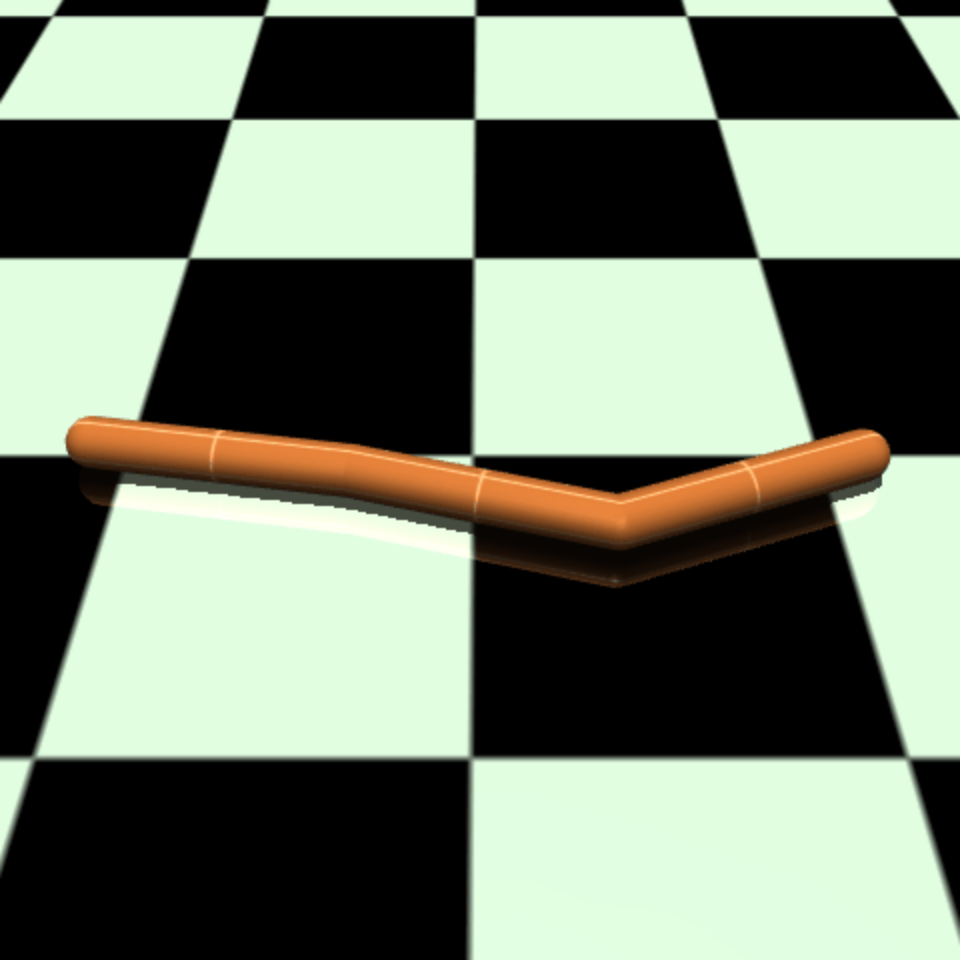
\includegraphics[width=0.18\linewidth]{figs/mujoco_swimmer.png}
    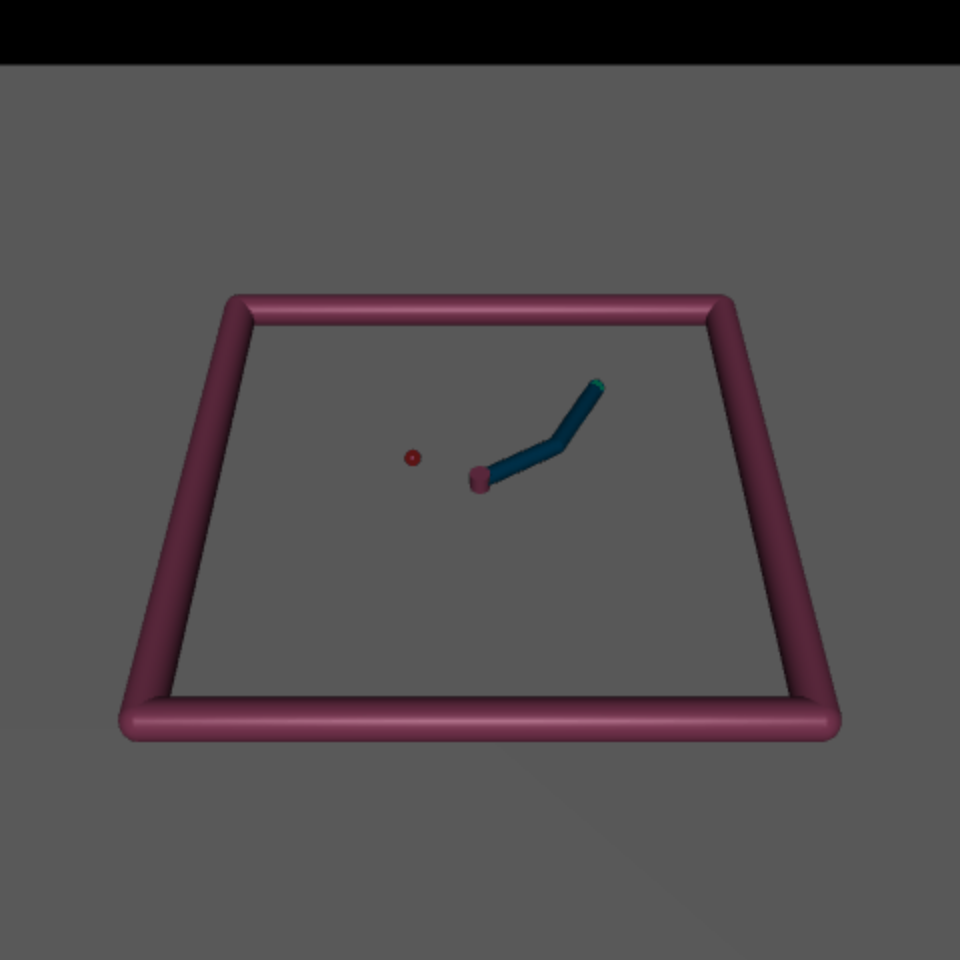
\includegraphics[width=0.18\linewidth]{figs/mujoco_reacher.png}
    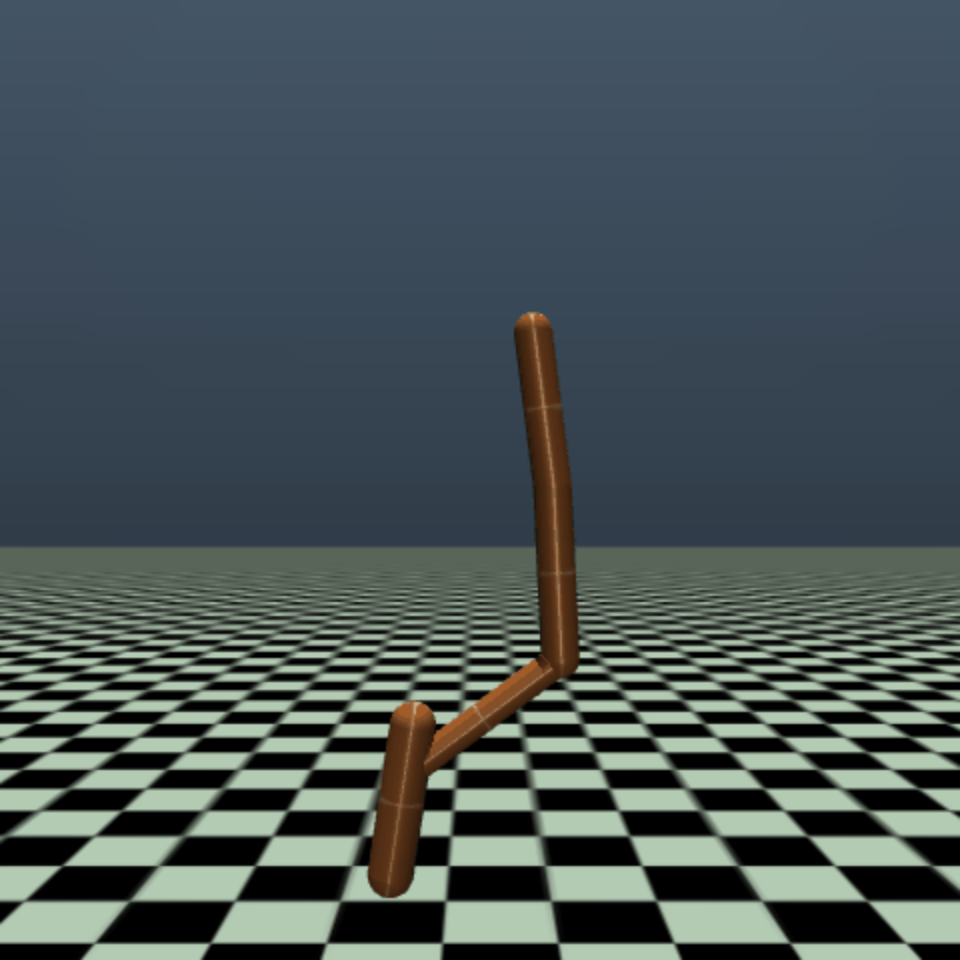
\includegraphics[width=0.18\linewidth]{figs/mujoco_hopper.png}
    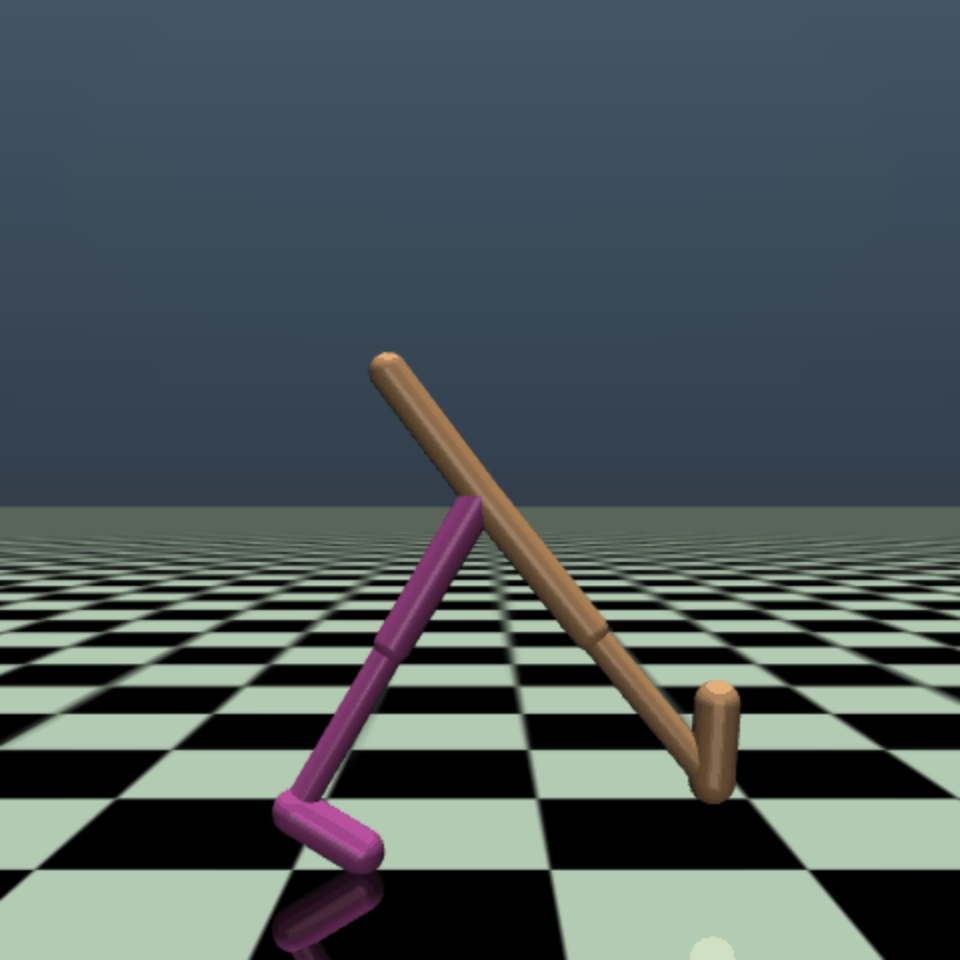
\includegraphics[width=0.18\linewidth]{figs/mujoco_walker.png}
    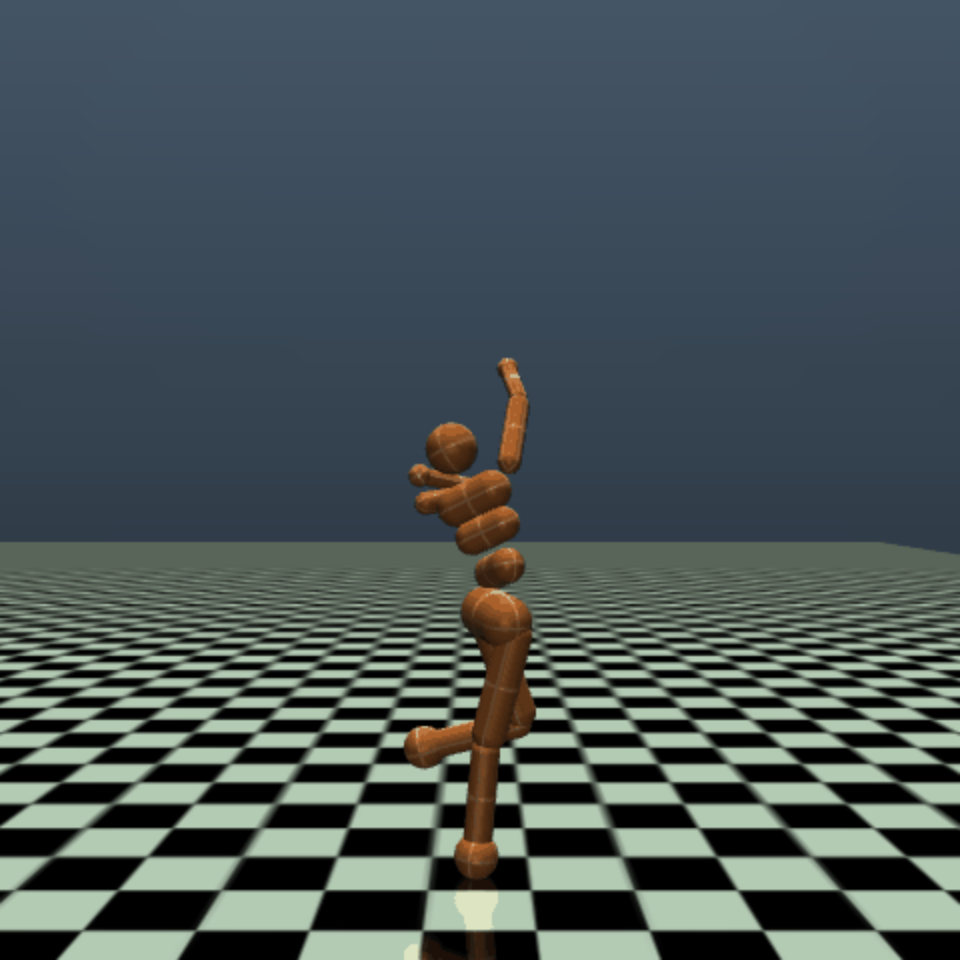
\includegraphics[width=0.18\linewidth]{figs/mujoco_humanoid.png}
    \caption{MuJoCo datasets: \textsc{Swimmer}, \textsc{Reacher}, \textsc{Hopper}, \textsc{Walker2d} and \textsc{Humanoid} environments (left to right).}
    \label{fig:dr4l}
\end{figure}
We provide comprehensive datasets for all MuJoCo \cite{mujoco} robotic tasks available in the Gymnasium package \cite{andreasthesis}. These datasets were generated using Stable Baselines 3 \cite{sb3}, primarily employing Soft Actor Critic \cite{sac}, with Truncated Quantile Critics \cite{tqc} used specifically for the complex \textsc{Humanoid} environment. By strategically early-stopping training at different performance plateaus, we created multiple dataset variants that capture diverse skill levels. These varied performance levels are important for evaluating algorithm robustness with imperfect datasets, better reflecting real-world applications.

For balancing tasks (\textsc{InvertedPendulum}, \textsc{InvertedDoublePendulum}), we offer expert datasets (perfect balance maintenance) and medium datasets (balance sustained for approximately 100 steps). Arm manipulation environments (\textsc{Reacher}, \textsc{Pusher}) similarly include expert variants (efficient goal achievement) and medium variants (suboptimal but functional performance).
Our 2D locomotion environments (\textsc{HalfCheetah}, \textsc{Hopper}, \textsc{Walker2D}) feature three performance tiers: expert (optimal natural motion), medium (competent but suboptimal movement), and simple (basic functional locomotion). The \textsc{Swimmer} environment includes expert (efficient serpentine motion) and medium (functional but inefficient movement) variants.
For more complex locomotion, \textsc{Ant} datasets span expert (fast galloping with occasional falls), medium (stable rapid walking), and simple (slow, highly stable movement) variants. \textsc{Humanoid} similarly provides expert (running), medium (brisk walking), and simple (slow, sliding movement) variants.

\subsection{BabyAI}
\begin{figure}[t!]
    \centering
    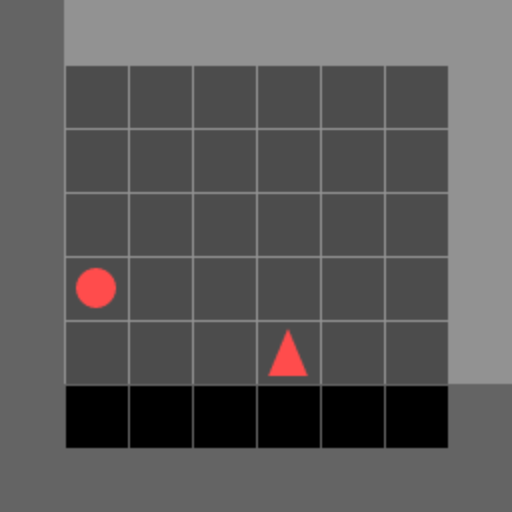
\includegraphics[width=0.18\linewidth]{figs/babyai_gotoredballnodists.png}
    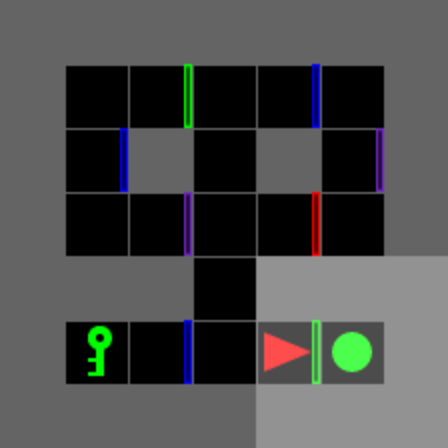
\includegraphics[width=0.18\linewidth]{figs/babyai_keycorridors3r3.png}
    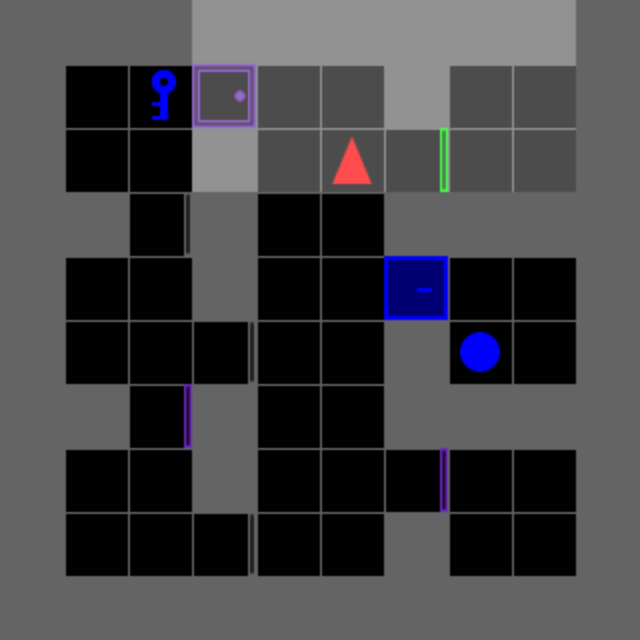
\includegraphics[width=0.18\linewidth]{figs/babyai_keycorridors4r3.png}
    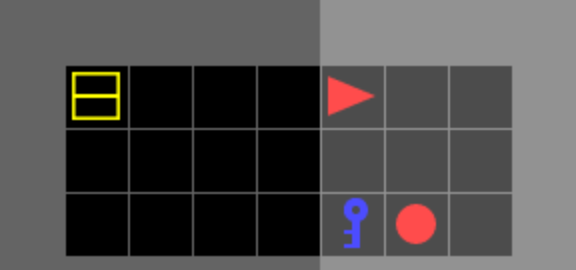
\includegraphics[width=0.384\linewidth]{figs/babyai_movetwoacrosss5n2.png}
    \caption{BabyAI datasets: \textsc{GoToRedBall}, \textsc{KeyCorridor} (two variants), and \textsc{MoveTwoAcross} tasks (left to right).}
    \label{fig:dr4l}
\end{figure}
BabyAI \cite{babyai} presents a suite of instruction-following tasks in grid world environments designed to study grounded language learning. These environments feature an agent that must interpret and execute natural language instructions in partially observable grid-based worlds. The tasks range from simple navigation commands to complex multi-step instructions involving object manipulation.

We generated 170 distinct datasets spanning the entire BabyAI task hierarchy, from basic GoToRedBall scenarios to complex instructions following in BossLevel. For each environment, we created two dataset variants: (1) with agent-centric partial observations that simulate a limited field of view, and (2) with full grid observations providing complete state information. This dual representation enables research on both partially observable and fully observable instruction-following tasks.

All trajectories were collected using the deterministic expert policy provided in the BabyAI framework, which generates optimal solutions for each task. Each dataset contains 1,000 complete episodes, ensuring sufficient data for training and evaluation. The datasets capture diverse linguistic instructions paired with the corresponding state-action trajectories required to fulfill them, providing a rich resource for studying language grounding, hierarchical planning, and instruction following in reinforcement learning.


\subsection{Atari}
\begin{figure}[t!]
    \centering
    
\includegraphics[width=0.18\linewidth]{figs/atari_breakout.png}
    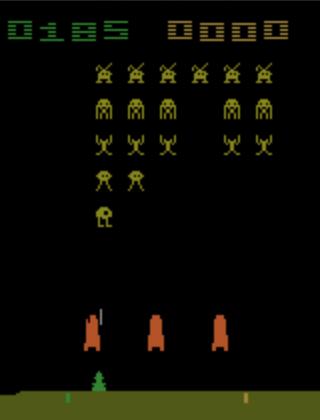
\includegraphics[width=0.18\linewidth]{figs/atari_spaceinvaders.png}
    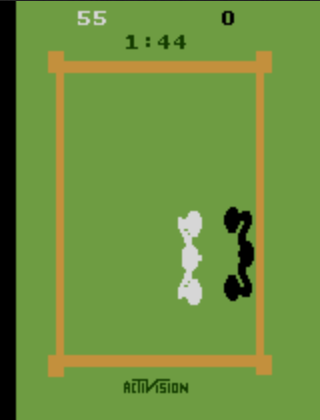
\includegraphics[width=0.18\linewidth]{figs/atari_boxing.png}
    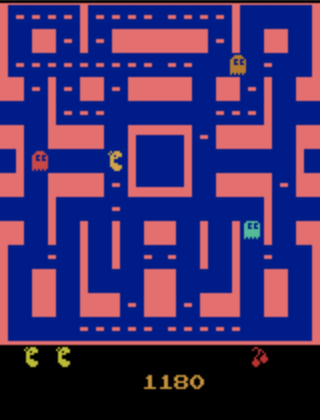
\includegraphics[width=0.18\linewidth]{figs/atari_mspacman.png}
    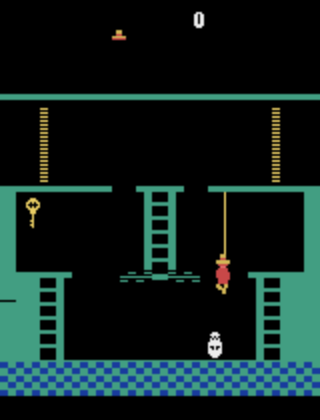
\includegraphics[width=0.18\linewidth]{figs/atari_montezuma.png}
    \caption{ALE datasets: \textsc{Breakout}, \textsc{Space Invaders}, \textsc{Boxing}, \textsc{Ms PacMan} and \textsc{Montezuma's Revenge} environments (left to right).}
    \label{fig:dr4l}
\end{figure}
The Arcade Learning Environment (ALE) \cite{ALE} serves as a foundational benchmark in reinforcement learning research. We collected expert demonstrations across 57 distinct Atari 2600 games, capturing diverse gameplay dynamics and challenge levels. For each environment, we recorded 10 complete episodes using pretrained agents from CleanRL \cite{cleanrl}, which implemented PPO \cite{ppo} with IMPALA architecture \cite{impala}. While the policy employs standard preprocessing techniques such as frame stacking, grayscale conversion, and resizing, the dataset preserves raw images as observations, allowing users the flexibility to apply their own preprocessing methods.

The collection spans diverse game types including shooting games (Space Invaders), maze navigation (Ms. Pac-Man), sports simulations (Boxing), and puzzle environments (Montezuma's Revenge). These datasets provide several unique characteristics that complement our other collections: pixel-based observations, longer temporal dependencies, diverse reward structures, and established performance benchmarks. This makes them particularly valuable for research in representation learning, credit assignment, and visual policy learning across the spectrum of reinforcement learning challenges.

% \subsection{\color{red}TODO: ManiSkill}
\subsection{MetaWorld}
MetaWorld \cite{metaworld} provides a benchmark of 50 diverse robotic manipulation tasks designed for multi-task and meta-reinforcement learning research. Each task features a simulated Sawyer robotic arm performing various operations (reaching, pushing, pick-and-place, tool use, door manipulation, and button pressing) within a MuJoCo environment. We generated datasets for all 50 tasks using the deterministic expert policies provided in the official MetaWorld package, collecting 50 complete episodes per task. These policies, developed using an heuristic controller, demonstrate near-optimal performance across environments.

The datasets preserve full state information, including the 3D hand position, end-effector configuration, object properties, and goal position. This makes them valuable for various research applications in offline reinforcement learning, transfer learning, and skill composition. Unlike the D4RL manipulation datasets that focus on high-dimensional dexterous manipulation, these datasets emphasize a wider variety of structured tasks with clearly defined success criteria.


\subsection{WebAgents}
We integrated WebLINX \cite{weblinx}, a large-scale dataset of web interactions, into the Minari format. WebLINX contains 24K interactions across 969 successful trajectories of agents completing tasks on the web. This dataset demonstrates Minari's broad applicability beyond traditional reinforcement learning scenarios, as it consists primarily of text-based observations and actions without explicit reward signals.

The trajectories capture diverse web navigation tasks, including form completion, information retrieval, and multi-step workflows across various websites. By supporting this dataset format, Minari enables researchers to easily test offline reinforcement learning techniques to web automation, text-based agents, and instruction following in browser environments.

\section{Conclusion}
This paper introduces Minari, an open-source library designed to address the important challenges of standardization, reproducibility, and interoperability in reinforcement learning datasets. By establishing a unified framework for collecting, manipulating, and sharing agent experience data, Minari significantly lowers the barriers to collaboration and accelerates progress in offline reinforcement learning research.

The library's feature set supports the entire dataset lifecycle, from initial collection to sharing and reuse. Its adherence to consistent naming conventions, detailed metadata, and flexible file formats ensures that datasets are both accessible and reproducible. The seamless integration with major offline reinforcement learning frameworks like TorchRL, AgileRL, and D3RLPY further enhances its utility within existing research workflows.

Our curated collection of 338 datasets spanning robotics, navigation, instruction following, Atari games, and web interactions provides a concrete resource for the research community, with 350K unique trajectories totaling 55M interaction steps. This diverse collection enables researchers to benchmark algorithms across multiple domains and complexity levels without the overhead of dataset generation and processing.

Despite these advantages, Minari has certain limitations. Since data is saved in episodes and read as batches of episodes, Minari may struggle with life-long episodes in open-ended tasks where clear episode boundaries are not defined. Additionally, while Minari relies on high-efficiency data formats, it might introduce overhead compared to highly-optimized training pipelines with specialized data loaders.

As we continue to expand Minari's capabilities and dataset collection, we envision it becoming a major infrastructure for advancing data-driven reinforcement learning. By standardizing the way agent experience is shared and reused, Minari aims to foster a more collaborative research ecosystem where insights and innovations can build upon each other more efficiently.

\begin{ack}
We acknowledge every contributor, please find the complete list here: https://github.com/Farama-Foundation/Minari/graphs/contributors
\end{ack}

\bibliographystyle{plainnat}
\bibliography{refs}


%%%%%%%%%%%%%%%%%%%%%%%%%%%%%%%%%%%%%%%%%%%%%%%%%%%%%%%%%%%%

\appendix


\section{Dataset Metadata}

Both datasets and individual episodes can have metadata attached to them. The dataset metadata can be specified by the user during dataset creation. When creating a Minari dataset the default global metadata will be the ones reported in Table \ref{tab:metadata}.

\begin{table}[H]
    \centering
    \begin{tabular}{lll}
    \toprule
        Attribute & Type & Description \\ \midrule
        \pythoninline{dataset_id} & \pythoninline{str} & Identifier of the Minari dataset. \\
        \pythoninline{total_episodes} & \pythoninline{int} & Number of episodes in the Minari dataset. \\
        \pythoninline{total_steps} & \pythoninline{int} & Number of steps in the Minari dataset. \\
        \pythoninline{action_space} & \pythoninline{Space} & Gymnasium action space describing actions in dataset. \\
        \pythoninline{observation_space} & \pythoninline{Space} & Gymnasium observation space describing observations in dataset. \\
        \pythoninline{env_spec} & \pythoninline{str} & JSON string of the Gymnasium environment spec. \\
        \pythoninline{code_permalink} & \pythoninline{str} & Link to a repository with the code used to generate the dataset. \\
        \pythoninline{author} & \pythoninline{set of str} & Name of the authors that created the dataset. \\
        \pythoninline{author_email} & \pythoninline{set of str} & Email of the authors that created the dataset. \\
        \pythoninline{algorithm_name} & \pythoninline{str} & Name of the expert policy used to create the dataset. \\
        \pythoninline{minari_version} & \pythoninline{str} & Version of Minari that generated the dataset. \\
        \pythoninline{requirements} & \pythoninline{list of str} & List of requirements in pip-style to load the environment. \\ \bottomrule
    \end{tabular}
    \caption{List of metadata attributes of a Minari dataset.}
    \label{tab:metadata}
\end{table}

Only \pythoninline{dataset_id}, \pythoninline{total_episodes}, and \pythoninline{total_steps} are mandatory (with the latter two automatically computed). Metadata for each episode is also supported and can be added by the user via a callback function. The episode statistics for the observed rewards are automatically computed.

\section{Environment support}

The Minari storage format supports the following observation and action spaces:

\begin{table}[H]
    \centering
    \begin{tabular}{lll}
        \toprule
        Space & Description & \\ \midrule
        \pythoninline{Box} & An n-dimensional continuous space. & \\
        \pythoninline{Discrete} & Describes a discrete space with an observation in $\{0, 1, ..., n-1\}$. & \\
        \pythoninline{MultiDiscrete} & Represents the cartesian product of arbitrary Discrete spaces. & \\
        \pythoninline{MultiBinary} & A binary space. The elements are binary arrays. & \\
        \pythoninline{Tuple} & Represents a tuple of spaces. & \\
        \pythoninline{Dict} & Represents a dictionary of spaces. & \\
        \pythoninline{Text} & The elements of this space are bounded strings from a charset. & \\ \bottomrule
    \end{tabular}
\end{table}

\section{Episode data structure}

A Minari dataset is encapsulated in the `MinariDataset` class which allows for iterating and sampling through episodes which are defined as \pythoninlin  e{EpisodeData} data class. Take the following example where we load the \pythoninline{D4RL/door/human-v2} dataset and randomly sample 10 episodes:

\begin{python}
import minari
dataset = minari.load_dataset("D4RL/door/human-v2", download=True)
sampled_episodes = dataset.sample_episodes(10)
\end{python}

The \pythoninline{sampled_episodes} variable will be a list of 10 \pythoninline{EpisodeData} elements, each containing episode data. An \pythoninline{EpisodeData} element is a data class consisting of the following fields:

\begin{table}[H]
    \centering
    \begin{tabular}{lll}
    \toprule
        Field & Type & Description \\ \midrule
        \pythoninline{id} & \pythoninline{int} & ID of the episode. \\
        \pythoninline{observations} & \pythoninline{np.ndarray}, \pythoninline{list}, \pythoninline{tuple}, \pythoninline{dict} & Stacked observations for each step. \\
        \pythoninline{actions} & \pythoninline{np.ndarray}, \pythoninline{list}, \pythoninline{tuple}, \pythoninline{dict} & Stacked actions for each step. \\
        \pythoninline{rewards} & \pythoninline{np.ndarray} & Rewards for each step. \\
        \pythoninline{terminations} & \pythoninline{np.ndarray} & Terminations for each step. \\
        \pythoninline{truncations} & \pythoninline{np.ndarray} & Truncations for each step. \\
        \pythoninline{infos} & \pythoninline{dict} & Additional information returned by the environment \\ \bottomrule
    \end{tabular}
\end{table}

where the specific type of the observation and action depends on their respective spaces.


\section*{NeurIPS Paper Checklist}


\begin{enumerate}

\item {\bf Claims}
    \item[] Question: Do the main claims made in the abstract and introduction accurately reflect the paper's contributions and scope?
    \item[] Answer: \answerYes{} % Replace by \answerYes{}, \answerNo{}, or \answerNA{}.
    \item[] Justification: We claim a new Python package, with a set of datasets which is the content of the paper.
    \item[] Guidelines:
    \begin{itemize}
        \item The answer NA means that the abstract and introduction do not include the claims made in the paper.
        \item The abstract and/or introduction should clearly state the claims made, including the contributions made in the paper and important assumptions and limitations. A No or NA answer to this question will not be perceived well by the reviewers. 
        \item The claims made should match theoretical and experimental results, and reflect how much the results can be expected to generalize to other settings. 
        \item It is fine to include aspirational goals as motivation as long as it is clear that these goals are not attained by the paper. 
    \end{itemize}

\item {\bf Limitations}
    \item[] Question: Does the paper discuss the limitations of the work performed by the authors?
    \item[] Answer: \answerYes{} % Replace by \answerYes{}, \answerNo{}, or \answerNA{}.
    \item[] Justification: Yes, we pointed out in the conclusions and in the introduction the limitations regarding the choice of episode batching for data and speed efficiency.
    \item[] Guidelines:
    \begin{itemize}
        \item The answer NA means that the paper has no limitation while the answer No means that the paper has limitations, but those are not discussed in the paper. 
        \item The authors are encouraged to create a separate "Limitations" section in their paper.
        \item The paper should point out any strong assumptions and how robust the results are to violations of these assumptions (e.g., independence assumptions, noiseless settings, model well-specification, asymptotic approximations only holding locally). The authors should reflect on how these assumptions might be violated in practice and what the implications would be.
        \item The authors should reflect on the scope of the claims made, e.g., if the approach was only tested on a few datasets or with a few runs. In general, empirical results often depend on implicit assumptions, which should be articulated.
        \item The authors should reflect on the factors that influence the performance of the approach. For example, a facial recognition algorithm may perform poorly when image resolution is low or images are taken in low lighting. Or a speech-to-text system might not be used reliably to provide closed captions for online lectures because it fails to handle technical jargon.
        \item The authors should discuss the computational efficiency of the proposed algorithms and how they scale with dataset size.
        \item If applicable, the authors should discuss possible limitations of their approach to address problems of privacy and fairness.
        \item While the authors might fear that complete honesty about limitations might be used by reviewers as grounds for rejection, a worse outcome might be that reviewers discover limitations that aren't acknowledged in the paper. The authors should use their best judgment and recognize that individual actions in favor of transparency play an important role in developing norms that preserve the integrity of the community. Reviewers will be specifically instructed to not penalize honesty concerning limitations.
    \end{itemize}

\item {\bf Theory assumptions and proofs}
    \item[] Question: For each theoretical result, does the paper provide the full set of assumptions and a complete (and correct) proof?
    \item[] Answer: \answerNA{} % Replace by \answerYes{}, \answerNo{}, or \answerNA{}.
    \item[] Justification: The paper doesn't provide any theoretical result.
    \item[] Guidelines:
    \begin{itemize}
        \item The answer NA means that the paper does not include theoretical results. 
        \item All the theorems, formulas, and proofs in the paper should be numbered and cross-referenced.
        \item All assumptions should be clearly stated or referenced in the statement of any theorems.
        \item The proofs can either appear in the main paper or the supplemental material, but if they appear in the supplemental material, the authors are encouraged to provide a short proof sketch to provide intuition. 
        \item Inversely, any informal proof provided in the core of the paper should be complemented by formal proofs provided in appendix or supplemental material.
        \item Theorems and Lemmas that the proof relies upon should be properly referenced. 
    \end{itemize}

    \item {\bf Experimental result reproducibility}
    \item[] Question: Does the paper fully disclose all the information needed to reproduce the main experimental results of the paper to the extent that it affects the main claims and/or conclusions of the paper (regardless of whether the code and data are provided or not)?
    \item[] Answer: \answerNA{} % Replace by \answerYes{}, \answerNo{}, or \answerNA{}.
    \item[] Justification: The paper doesn't provide any experiments.
    \item[] Guidelines:
    \begin{itemize}
        \item The answer NA means that the paper does not include experiments.
        \item If the paper includes experiments, a No answer to this question will not be perceived well by the reviewers: Making the paper reproducible is important, regardless of whether the code and data are provided or not.
        \item If the contribution is a dataset and/or model, the authors should describe the steps taken to make their results reproducible or verifiable. 
        \item Depending on the contribution, reproducibility can be accomplished in various ways. For example, if the contribution is a novel architecture, describing the architecture fully might suffice, or if the contribution is a specific model and empirical evaluation, it may be necessary to either make it possible for others to replicate the model with the same dataset, or provide access to the model. In general. releasing code and data is often one good way to accomplish this, but reproducibility can also be provided via detailed instructions for how to replicate the results, access to a hosted model (e.g., in the case of a large language model), releasing of a model checkpoint, or other means that are appropriate to the research performed.
        \item While NeurIPS does not require releasing code, the conference does require all submissions to provide some reasonable avenue for reproducibility, which may depend on the nature of the contribution. For example
        \begin{enumerate}
            \item If the contribution is primarily a new algorithm, the paper should make it clear how to reproduce that algorithm.
            \item If the contribution is primarily a new model architecture, the paper should describe the architecture clearly and fully.
            \item If the contribution is a new model (e.g., a large language model), then there should either be a way to access this model for reproducing the results or a way to reproduce the model (e.g., with an open-source dataset or instructions for how to construct the dataset).
            \item We recognize that reproducibility may be tricky in some cases, in which case authors are welcome to describe the particular way they provide for reproducibility. In the case of closed-source models, it may be that access to the model is limited in some way (e.g., to registered users), but it should be possible for other researchers to have some path to reproducing or verifying the results.
        \end{enumerate}
    \end{itemize}


\item {\bf Open access to data and code}
    \item[] Question: Does the paper provide open access to the data and code, with sufficient instructions to faithfully reproduce the main experimental results, as described in supplemental material?
    \item[] Answer: \answerYes{} % Replace by \answerYes{}, \answerNo{}, or \answerNA{}.
    \item[] Justification: Yes, the Python package is open-source and available on GitHub. The data is publicly available on HuggingFace.
    \item[] Guidelines:
    \begin{itemize}
        \item The answer NA means that paper does not include experiments requiring code.
        \item Please see the NeurIPS code and data submission guidelines (\url{https://nips.cc/public/guides/CodeSubmissionPolicy}) for more details.
        \item While we encourage the release of code and data, we understand that this might not be possible, so “No” is an acceptable answer. Papers cannot be rejected simply for not including code, unless this is central to the contribution (e.g., for a new open-source benchmark).
        \item The instructions should contain the exact command and environment needed to run to reproduce the results. See the NeurIPS code and data submission guidelines (\url{https://nips.cc/public/guides/CodeSubmissionPolicy}) for more details.
        \item The authors should provide instructions on data access and preparation, including how to access the raw data, preprocessed data, intermediate data, and generated data, etc.
        \item The authors should provide scripts to reproduce all experimental results for the new proposed method and baselines. If only a subset of experiments are reproducible, they should state which ones are omitted from the script and why.
        \item At submission time, to preserve anonymity, the authors should release anonymized versions (if applicable).
        \item Providing as much information as possible in supplemental material (appended to the paper) is recommended, but including URLs to data and code is permitted.
    \end{itemize}


\item {\bf Experimental setting/details}
    \item[] Question: Does the paper specify all the training and test details (e.g., data splits, hyperparameters, how they were chosen, type of optimizer, etc.) necessary to understand the results?
    \item[] Answer: \answerNA{} % Replace by \answerYes{}, \answerNo{}, or \answerNA{}.
    \item[] Justification:The paper doesn't present any training.
    \item[] Guidelines:
    \begin{itemize}
        \item The answer NA means that the paper does not include experiments.
        \item The experimental setting should be presented in the core of the paper to a level of detail that is necessary to appreciate the results and make sense of them.
        \item The full details can be provided either with the code, in appendix, or as supplemental material.
    \end{itemize}

\item {\bf Experiment statistical significance}
    \item[] Question: Does the paper report error bars suitably and correctly defined or other appropriate information about the statistical significance of the experiments?
    \item[] Answer: \answerNA{} % Replace by \answerYes{}, \answerNo{}, or \answerNA{}.
    \item[] Justification: We did not present any information which needed statistical analysis.
    \item[] Guidelines:
    \begin{itemize}
        \item The answer NA means that the paper does not include experiments.
        \item The authors should answer "Yes" if the results are accompanied by error bars, confidence intervals, or statistical significance tests, at least for the experiments that support the main claims of the paper.
        \item The factors of variability that the error bars are capturing should be clearly stated (for example, train/test split, initialization, random drawing of some parameter, or overall run with given experimental conditions).
        \item The method for calculating the error bars should be explained (closed form formula, call to a library function, bootstrap, etc.)
        \item The assumptions made should be given (e.g., Normally distributed errors).
        \item It should be clear whether the error bar is the standard deviation or the standard error of the mean.
        \item It is OK to report 1-sigma error bars, but one should state it. The authors should preferably report a 2-sigma error bar than state that they have a 96\% CI, if the hypothesis of Normality of errors is not verified.
        \item For asymmetric distributions, the authors should be careful not to show in tables or figures symmetric error bars that would yield results that are out of range (e.g. negative error rates).
        \item If error bars are reported in tables or plots, The authors should explain in the text how they were calculated and reference the corresponding figures or tables in the text.
    \end{itemize}

\item {\bf Experiments compute resources}
    \item[] Question: For each experiment, does the paper provide sufficient information on the computer resources (type of compute workers, memory, time of execution) needed to reproduce the experiments?
    \item[] Answer: \answerNA{} % Replace by \answerYes{}, \answerNo{}, or \answerNA{}.
    \item[] Justification: We didn't present any experiments which need particular compute resources.
    \item[] Guidelines:
    \begin{itemize}
        \item The answer NA means that the paper does not include experiments.
        \item The paper should indicate the type of compute workers CPU or GPU, internal cluster, or cloud provider, including relevant memory and storage.
        \item The paper should provide the amount of compute required for each of the individual experimental runs as well as estimate the total compute. 
        \item The paper should disclose whether the full research project required more compute than the experiments reported in the paper (e.g., preliminary or failed experiments that didn't make it into the paper). 
    \end{itemize}
    
\item {\bf Code of ethics}
    \item[] Question: Does the research conducted in the paper conform, in every respect, with the NeurIPS Code of Ethics \url{https://neurips.cc/public/EthicsGuidelines}?
    \item[] Answer: \answerYes{} % Replace by \answerYes{}, \answerNo{}, or \answerNA{}.
    \item[] Justification: The paper doesn't perform any crowdsourcing; the data comes from controlled simulated environments, so it is not harmful nor violate privacy; it doesn't have safety risks.
    \item[] Guidelines:
    \begin{itemize}
        \item The answer NA means that the authors have not reviewed the NeurIPS Code of Ethics.
        \item If the authors answer No, they should explain the special circumstances that require a deviation from the Code of Ethics.
        \item The authors should make sure to preserve anonymity (e.g., if there is a special consideration due to laws or regulations in their jurisdiction).
    \end{itemize}


\item {\bf Broader impacts}
    \item[] Question: Does the paper discuss both potential positive societal impacts and negative societal impacts of the work performed?
    \item[] Answer: \answerYes{} % Replace by \answerYes{}, \answerNo{}, or \answerNA{}.
    \item[] Justification: Yes, we discuss the potential positive impact in fostering collaboration; we do not foresee any negative impact.
    \item[] Guidelines:
    \begin{itemize}
        \item The answer NA means that there is no societal impact of the work performed.
        \item If the authors answer NA or No, they should explain why their work has no societal impact or why the paper does not address societal impact.
        \item Examples of negative societal impacts include potential malicious or unintended uses (e.g., disinformation, generating fake profiles, surveillance), fairness considerations (e.g., deployment of technologies that could make decisions that unfairly impact specific groups), privacy considerations, and security considerations.
        \item The conference expects that many papers will be foundational research and not tied to particular applications, let alone deployments. However, if there is a direct path to any negative applications, the authors should point it out. For example, it is legitimate to point out that an improvement in the quality of generative models could be used to generate deepfakes for disinformation. On the other hand, it is not needed to point out that a generic algorithm for optimizing neural networks could enable people to train models that generate Deepfakes faster.
        \item The authors should consider possible harms that could arise when the technology is being used as intended and functioning correctly, harms that could arise when the technology is being used as intended but gives incorrect results, and harms following from (intentional or unintentional) misuse of the technology.
        \item If there are negative societal impacts, the authors could also discuss possible mitigation strategies (e.g., gated release of models, providing defenses in addition to attacks, mechanisms for monitoring misuse, mechanisms to monitor how a system learns from feedback over time, improving the efficiency and accessibility of ML).
    \end{itemize}
    
\item {\bf Safeguards}
    \item[] Question: Does the paper describe safeguards that have been put in place for responsible release of data or models that have a high risk for misuse (e.g., pretrained language models, image generators, or scraped datasets)?
    \item[] Answer: \answerNA{} % Replace by \answerYes{}, \answerNo{}, or \answerNA{}.
    \item[] Justification: As the data comes from controlled simulated environments, it doesn't have high risk of misuse.
    \item[] Guidelines:
    \begin{itemize}
        \item The answer NA means that the paper poses no such risks.
        \item Released models that have a high risk for misuse or dual-use should be released with necessary safeguards to allow for controlled use of the model, for example by requiring that users adhere to usage guidelines or restrictions to access the model or implementing safety filters. 
        \item Datasets that have been scraped from the Internet could pose safety risks. The authors should describe how they avoided releasing unsafe images.
        \item We recognize that providing effective safeguards is challenging, and many papers do not require this, but we encourage authors to take this into account and make a best faith effort.
    \end{itemize}

\item {\bf Licenses for existing assets}
    \item[] Question: Are the creators or original owners of assets (e.g., code, data, models), used in the paper, properly credited and are the license and terms of use explicitly mentioned and properly respected?
    \item[] Answer: \answerYes{} % Replace by \answerYes{}, \answerNo{}, or \answerNA{}.
    \item[] Justification: Yes, for existing data, such as weblinx, we mentioned the authors and respected the license.
    \item[] Guidelines:
    \begin{itemize}
        \item The answer NA means that the paper does not use existing assets.
        \item The authors should cite the original paper that produced the code package or dataset.
        \item The authors should state which version of the asset is used and, if possible, include a URL.
        \item The name of the license (e.g., CC-BY 4.0) should be included for each asset.
        \item For scraped data from a particular source (e.g., website), the copyright and terms of service of that source should be provided.
        \item If assets are released, the license, copyright information, and terms of use in the package should be provided. For popular datasets, \url{paperswithcode.com/datasets} has curated licenses for some datasets. Their licensing guide can help determine the license of a dataset.
        \item For existing datasets that are re-packaged, both the original license and the license of the derived asset (if it has changed) should be provided.
        \item If this information is not available online, the authors are encouraged to reach out to the asset's creators.
    \end{itemize}

\item {\bf New assets}
    \item[] Question: Are new assets introduced in the paper well documented and is the documentation provided alongside the assets?
    \item[] Answer: \answerYes{} % Replace by \answerYes{}, \answerNo{}, or \answerNA{}.
    \item[] Justification: Yes, Minari is a well-documented package, as well as its datasets; see: https://minari.farama.org
    \item[] Guidelines:
    \begin{itemize}
        \item The answer NA means that the paper does not release new assets.
        \item Researchers should communicate the details of the dataset/code/model as part of their submissions via structured templates. This includes details about training, license, limitations, etc. 
        \item The paper should discuss whether and how consent was obtained from people whose asset is used.
        \item At submission time, remember to anonymize your assets (if applicable). You can either create an anonymized URL or include an anonymized zip file.
    \end{itemize}

\item {\bf Crowdsourcing and research with human subjects}
    \item[] Question: For crowdsourcing experiments and research with human subjects, does the paper include the full text of instructions given to participants and screenshots, if applicable, as well as details about compensation (if any)? 
    \item[] Answer: \answerNA{} % Replace by \answerYes{}, \answerNo{}, or \answerNA{}.
    \item[] Justification: We don't make use of any crowdsourcing.
    \item[] Guidelines:
    \begin{itemize}
        \item The answer NA means that the paper does not involve crowdsourcing nor research with human subjects.
        \item Including this information in the supplemental material is fine, but if the main contribution of the paper involves human subjects, then as much detail as possible should be included in the main paper. 
        \item According to the NeurIPS Code of Ethics, workers involved in data collection, curation, or other labor should be paid at least the minimum wage in the country of the data collector. 
    \end{itemize}

\item {\bf Institutional review board (IRB) approvals or equivalent for research with human subjects}
    \item[] Question: Does the paper describe potential risks incurred by study participants, whether such risks were disclosed to the subjects, and whether Institutional Review Board (IRB) approvals (or an equivalent approval/review based on the requirements of your country or institution) were obtained?
    \item[] Answer: \answerNA{} % Replace by \answerYes{}, \answerNo{}, or \answerNA{}.
    \item[] Justification: We do not employ any human subject.
    \item[] Guidelines:
    \begin{itemize}
        \item The answer NA means that the paper does not involve crowdsourcing nor research with human subjects.
        \item Depending on the country in which research is conducted, IRB approval (or equivalent) may be required for any human subjects research. If you obtained IRB approval, you should clearly state this in the paper. 
        \item We recognize that the procedures for this may vary significantly between institutions and locations, and we expect authors to adhere to the NeurIPS Code of Ethics and the guidelines for their institution. 
        \item For initial submissions, do not include any information that would break anonymity (if applicable), such as the institution conducting the review.
    \end{itemize}

\item {\bf Declaration of LLM usage}
    \item[] Question: Does the paper describe the usage of LLMs if it is an important, original, or non-standard component of the core methods in this research? Note that if the LLM is used only for writing, editing, or formatting purposes and does not impact the core methodology, scientific rigorousness, or originality of the research, declaration is not required.
    %this research? 
    \item[] Answer: \answerNA{} % Replace by \answerYes{}, \answerNo{}, or \answerNA{}.
    \item[] Justification: We don't use any LLM, except for polishing the text.
    \item[] Guidelines:
    \begin{itemize}
        \item The answer NA means that the core method development in this research does not involve LLMs as any important, original, or non-standard components.
        \item Please refer to our LLM policy (\url{https://neurips.cc/Conferences/2025/LLM}) for what should or should not be described.
    \end{itemize}

\end{enumerate}

\end{document}
